\section*{Risk Treatment}
\addcontentsline{toc}{section}{Risk Treatment}

This part of the assessment aims at proposing a set of pre and post-incident security controls that can be found in figure \ref{fig:riskTreatCut2}. These controls are needed to lower the impact and the likelihood of an incident.

Regarding the main threats listed in the above section, the following main security controls were proposed

\begin{itemize}
    \item for \texttt{unauthorized wired connections} an intrusion prevention system to reduce the likelihood, and IP blacklist as post-control to reduce impact and avoid APT.
    \item for \texttt{hyperjacking} it is advisable to deploy the latest version of the hypervisor, implement a logical separation between guest and host machines, backup the configuration, and manage the hypervisor on a different port than the one used for hypervisor-guest communication\cite{online:virtualSec}. As post-controls, we can try and reset the admin credential, and restore the virtualization server with its backup, but if the access control is broken, then disaster recovery is needed.
    \item for \texttt{theft of equipment} the pre-controls consist of installing CCTV cameras, biometrical access control, and log personnel access. Since it's not reasonable to ask a municipality to install biometrical access control on a room that is used only when we are near the elections, we substituted this with a security officer.\cite{online:roomSec}
    \item for \texttt{router crashes} the main mitigations consist of implementing VRRP (Virtual Router Redundancy Protocol) \cite{online:VRRP} and configuration backup and restore when needed.
    \item finally, for \texttt{phishing campaigns} we need to train the personnel and implement anti-spam software on mail agents and SMTP servers to reduce the likelihood.
\end{itemize}

\begin{figure}[b!]
    \centering
    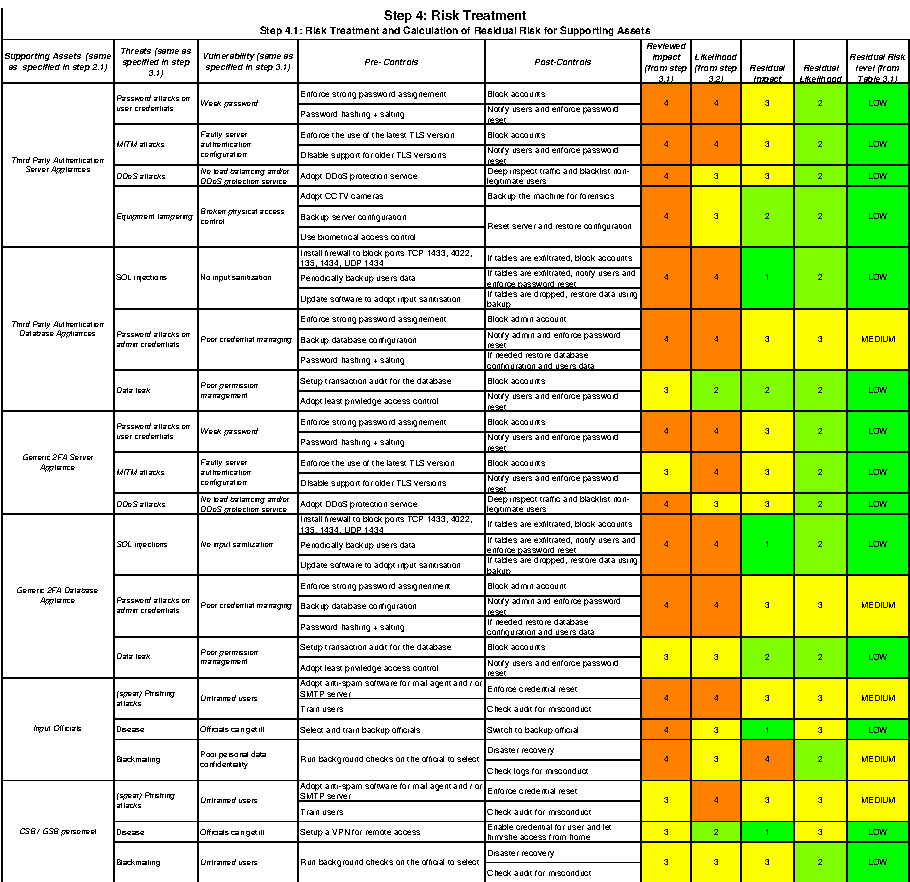
\includegraphics[keepaspectratio,width=1\textwidth]{03-risk-analysis/005-RT/img/riskTreatCut1.pdf}
    \label{fig:riskTreatCut1}
\end{figure}

\begin{figure}[t!]
    \centering
    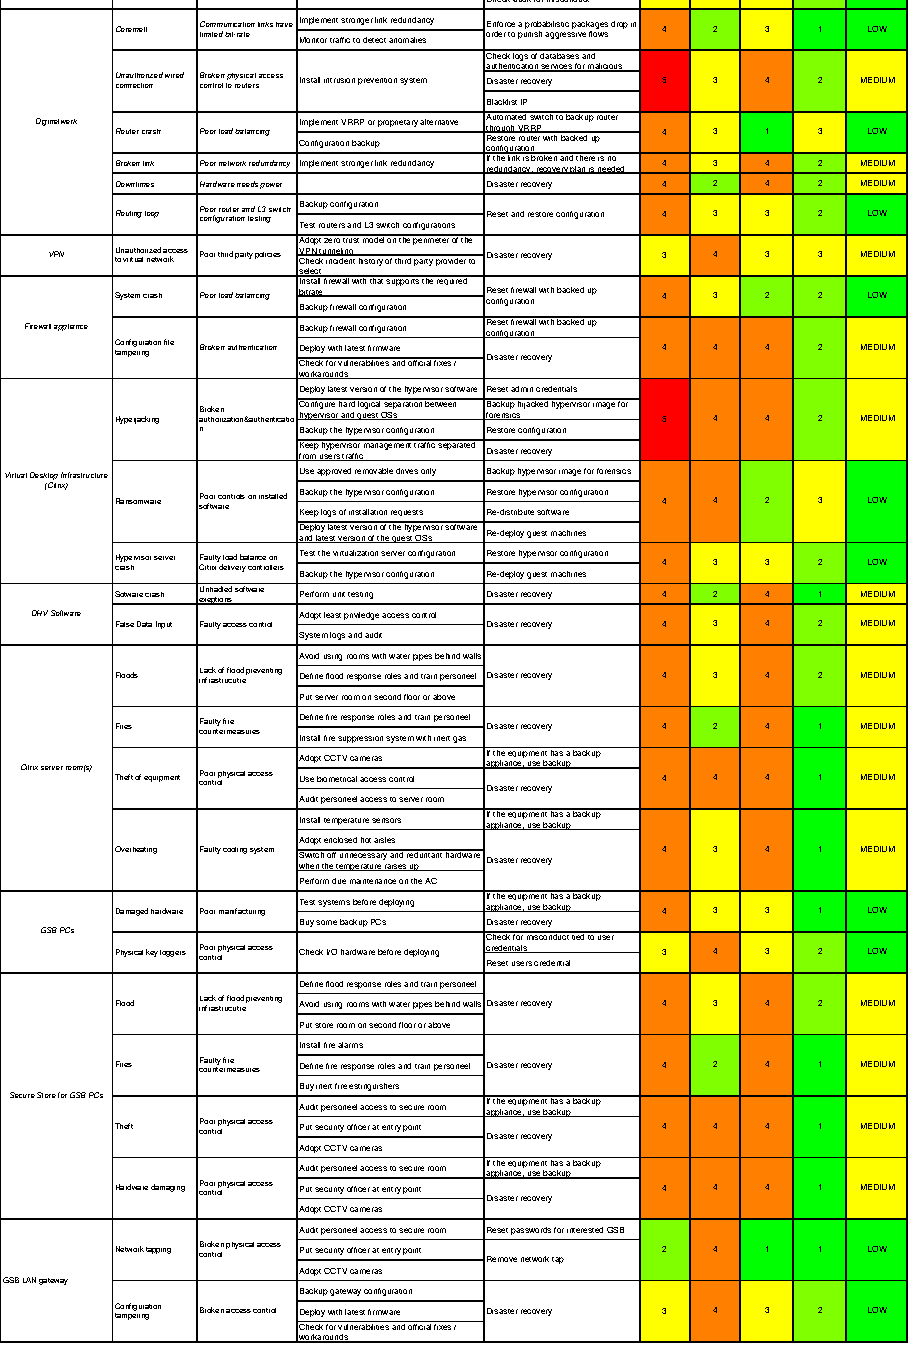
\includegraphics[keepaspectratio,width=1\textwidth]{03-risk-analysis/005-RT/img/riskTreatCut2.pdf}
    \caption{Risk treatment}
    \label{fig:riskTreatCut2}
\end{figure}

At the end of this step, no threats with high risk rating remained.\\

\noindent \textcolor{blue}{Update:}

\subsection*{Session Hijacking - CVE-2021-22927}

Citrix systems Inc. has already released an official patch with a reference guide on how to configure SAML. For this reason the vulnerability can be removed by upgrading the Citrix ADC software to version \texttt{13.0-82.41} or later, and by following the official configuration guide. \footnote{\href{https://support.citrix.com/article/CTX316577/citrix-application-delivery-controller-and-citrix-gateway-saml-configuration-reference-guide} {https://support.citrix.com/article/CTX316577/citrix-application-delivery-controller-and-citrix-gateway-saml-\\configuration-reference-guide}}

As a result, the impact is nulled.

\subsection*{Reverse Shell Attack - CVE-2022-38652}

It is stated in the vulnerability description that the affected products are in their EOL (End-of-Life) stage. No official patches or workarounds are available. As a first approach, the deployment of a DPI firewall was taken into consideration. More specifically, the goal was to whitelist only the necessary ports in order to block the instantiation of sockets used to expose the reversed shell. 

Unfortunately, not only this mitigation is too shallow since it only modifies the MAV metric, but also it can be bypassed. In fact, if an attacker has \texttt{SYSTEM} privileges on the victim machine, he/she could kill a process running on a whitelisted port and start an SSH session on that socket. Furthermore, to break the deep packet inspection, an adversary could tunnel the SSH session through a full TLS connection.\cite{online:SSH-TLS}

The vulnerability is reported to exists only in the software version for Windows systems. We suggest two approaches that depends on the production environment:

\begin{itemize}
    \item \textbf{deploy the software on a container running a Linux based OS}; this can be done by setting docker option \texttt{--ipc=host}. Note that this option drops the security requirements of the container and need to be tested.
    \item \textbf{replace Windows host with a Linux based OS}; this solution is more time consuming but it's the safest since it has been confirmed that the vulnerability does not exists in this environment.
\end{itemize}

To comply with our strict security policy, the second suggested solution is strongly advised as it surely nulls the impact of the threat.
